%
% (example1.tex)  2020.05.03 溝口佳寛
%
\documentclass[dvipdfmx]{jarticle}
%
\usepackage{graphicx,amsmath,amssymb}
\newtheorem{problem}{{\bf 問題}}
\title{LaTeXの練習}
\author{自分の名前に変える}
\西暦
\date{\today}

\begin{document}
\maketitle

\begin{problem}
放物線$y=x^2-2$と直線$y=x$で囲まれた部分の面積を求めなさい.
 \begin{center}
 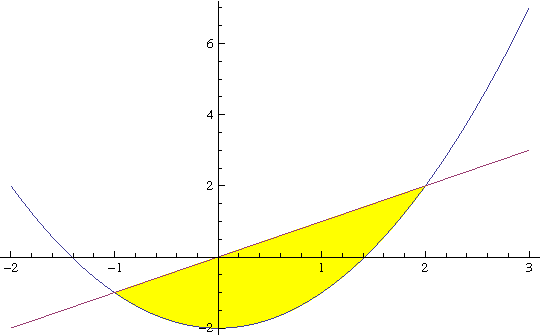
\includegraphics[scale=0.5]{fig1.pdf}
 \end{center}
\end{problem}

\noindent
{\bf [解答]} 交点の$x$座標を求める.
\begin{eqnarray*}
x^2-2 &=& x \\
x^2-x-2 &=& 0 \\
(x+1)(x-2)&=& 0
\end{eqnarray*}
より, 交点の$x$座標は $x=-1$ と $x=2$ である.

\begin{eqnarray*}
\int_{-1}^{2} x-(x^2 -2) \, dx &=& 
\int_{-1}^{2} -x^2 + x +2 \, dx \\
&=& \left[ -\frac{1}{3} x^3 + \frac{1}{2} x^2 + 2x \right]_{-1}^{2} \\
&=& (-\frac{1}{3} \cdot 2^3 + \frac{1}{2} \cdot 2^2 +2 \cdot 2 )
- (-\frac{1}{3} \cdot (-1)^3+\frac{1}{2} \cdot (-1)^2 +2 \cdot(-1)) \\
&=& -\frac{1}{3}(8+1) +\frac{1}{2}(4-1) +2(2+1) \\
&=& -3 + \frac{3}{2} + 6 \\
&=& \frac{9}{2}
\end{eqnarray*}

\begin{flushright}
\underline{{\bf 答.} 求める面積は $\displaystyle \frac{9}{2}$ である.}
\end{flushright}

\end{document}
